
\chapter{Basics}
\label{basics} 

Okay, I'm still working on my own understanding here, so, this is not etched
in stone.


\section{Hello, World}
\label{hello}

You knew it was coming.  You expected it.  You'd've been disappointed by its
absence.

%TODO  do this right, dammit

A basic \LaTeX document, article-style:

%TODO  Figure out how to get 80 columns to fit inside this box.  Smaller
% font?
\lstinputlisting[language=TeX,numbers=left]{hello.tex}

Until I get better, you're gonna want to grab the file yourself and compile
using \texttt{pdflatex} , see what the output looks like.

%\hline
%% hello.tex - simple example using the article
%
% 
\documentclass[a4paper,12pt,titlepage]{article}
\pagestyle{plain}
\title{Hello, World}
\author{Kurt Schmidt \\
	Drexel, Computer Science}
\date{Sept. 2014}

\begin{document}
\maketitle

Here's your obligatory `hello':  ``Hello.  Welcome to \LaTeX.''  \TeX is the
basic language, Developed by Donald Knuth.  \LaTeX is a way handy extension
to \TeX.  So, basic syntax probably applies to both.  Once we get into
packages, I've not clue, as yet, so, I'll just be talking about \LaTeX.

Easiest way to compile to PDF is using \texttt{pdflatex}.

\section{Math}
\label{hellomath}

And now, some math.  Remember, $\sum_{i=1}^m i = \frac{m(m+1)}{2}$, along
with identities for sums, and the sum of a geometric series.  You'll be
needing them.

Also recall these gems, you'll be needing them, too:

\[ b^{\log_{b}{x}} = x \]
\[ \log_{b}{b^x} = x \]
\[ \log_{b}{xy} = \log_{b}{x} + \log_{b}{y} \]
\[ \log_{b}{x/y} = \log_{b}{x} - \log_{b}{y} \]
\[ \log_{b}{x^n} = n\log_{b}{x} \]

So, 

\[ x^{\log_{b}{y}} = y^{\log_{b}{x}} \]

\section*{El Fin du Monde}
\label{end}

And that's it for now.  See section \ref{hellomath}.

\end{document}

%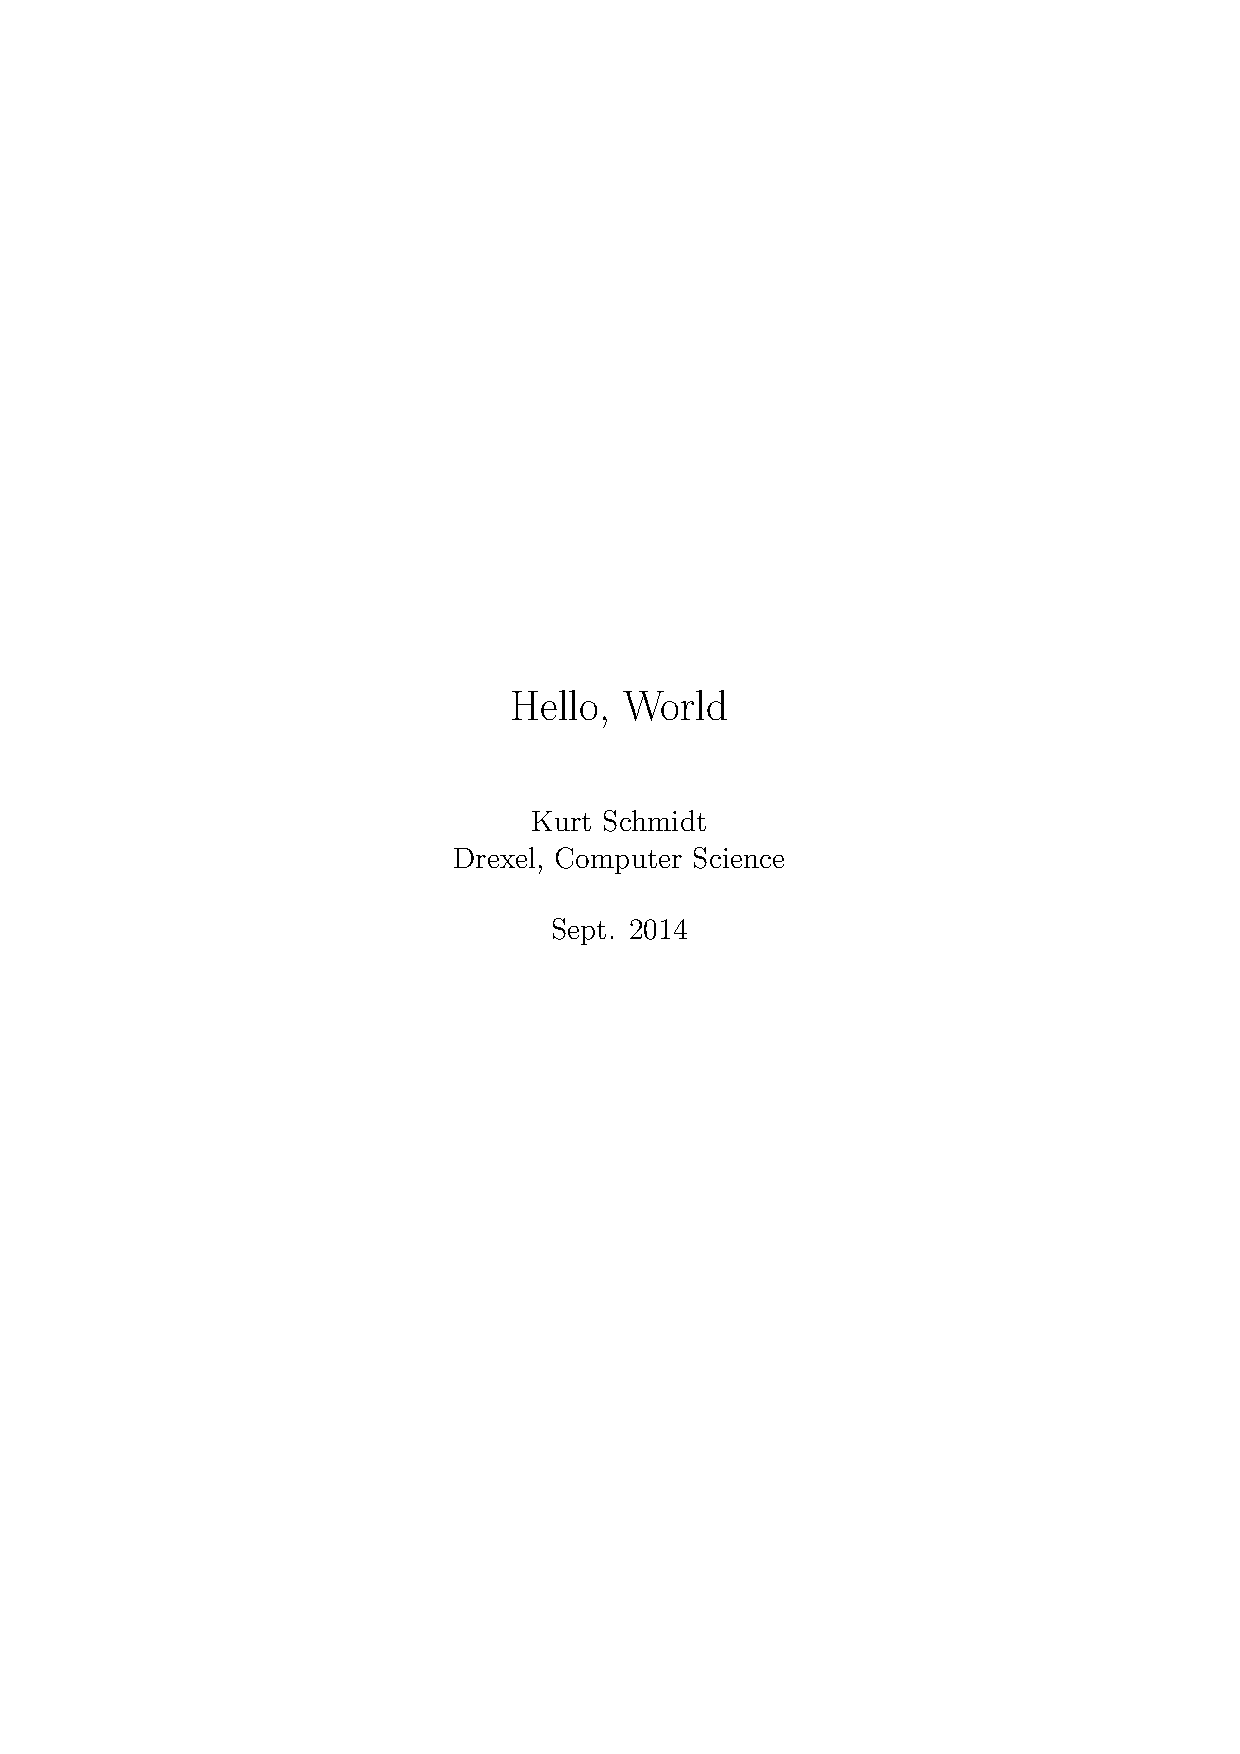
\includepdf{hello.pdf}

\section{Modes}
\label{modes-intro}

\TeX supports 2 basic modes, math and text.

When you're typing along, you're entering text.  Mostly you can just type as
you would, with a few exceptions.  There are metacharacters, paragraphs are
separated by two (or more) newlines.  We'll also want to talk about quotes,
hyphens and spaces.

Lines 24 and 30-34, in our hello example, show some uses of math mode.
See Section \ref{math} for a bit longer discussion.


\section{Metacharacters}
\label{metacharacters}

The following characters can not simply be typed, as they have special
meaning to \LaTeX{}:

\begin{quote}
	\{~~\}~~\$~~\%~~\_~~\&~~\#~~\^{}~~\textbackslash{}~~\~{}
\end{quote}

Here is how to print these characters in \LaTeX{}.  These metacharacters
will be explained, but for the moment, trust me.

\begin{center}
	\begin{tabular}{|c|l|}
		\hline
			\bf{Symbol} & \bf{\TeX sequence} \\
		\hline
			\{ & \textbackslash{}\{ \\
		\hline
			\} & \textbackslash{}\} \\
		\hline
			\$ & \textbackslash{}\$ \\
		\hline
			\% & \textbackslash{}\% \\
		\hline
			\& & \textbackslash{}\& \\
		\hline
			\# & \textbackslash{}\# \\
		\hline
			\_ & \textbackslash{}\_ \\
		\hline
			\textbackslash & \textbackslash{}textbackslash \\
		\hline
			\'{} & \textbackslash{}\'{}\{\} \\
		\hline
			\`{} & \textbackslash{}\`{}\{\} \\
		\hline
			\^{} & \textbackslash{}\^{}\{\} \\
		\hline
			\~{} & \textbackslash{}\~{}\{\} \\
			\textasciitilde & \textbackslash{}textasciitilde \\
			$\sim$ & \$\textbackslash{}sim\$ \\
		\hline
	\end{tabular}
\end{center}


\subsection{Braces for Grouping}

\{ \} are used for grouping.  Empty braces can be used to protect a special
symbol from immediate following text.  E.g.,
\texttt{\textbackslash{}textbackslash\{\}foo} would display
\textbackslash{}foo , since \texttt{\textbackslash{}textbackslashfoo} isn't
a character.


\subsection{Spaces}

Whitespace serves to separate words, etc, but in a typeset environment,
sequences of spaces, e.g., aren't of fixed size.

The \~{} in \LaTeX is a \emph{non-breaking space}.

If\textvisiblespace{}you\textvisiblespace{}want\textvisiblespace{}visible\textvisiblespace{}spaces,
use \textbackslash{}textvisiblespace\{\}.


\subsection{Quotes}
\label{basicquotes}

\LaTeX uses \`{}\`{} for left double quote, and \'{}\'{} for right double quote.
Similarly, \`{} and \'{} are used for left and right single quotes.

George said, `I heard an oldtimer once exclaim ``Oh, batshit!''{}'


\subsection{Dashes and Hyphens}

I believe the solitary \texttt{ - } is okay, though it might signal a
wordsplit, so, keep it in mind, if you have problems.  Well, let's see:
jack-in-the-box .

Two hyphens, \texttt{ -{}- }, yields an endash, --, and three, \texttt{
	-{}-{}- },  will give you an emdash, ---.

So, if you want 2 or more literal adjacent hyphens, -{}-, to keep the
sequence from being interpreted, use an empty string to separate them:
\texttt{ -\{\}-\{\}- } yields -{}-{}- .


\section{Special Characters}
\label{specchars}

Even if I knew what I was doing, this is a messy area.  For sanity's sake,
you want to restrict yourself to the 7-bit ASCII characters, and use \LaTeX
to create other characters.

You can change input encodings, \texttt{latin1}, \texttt{utf8}, etc., and
we're already past what I know.

We can represent many characters using escape codes.  Some special
characters are recognised in text mode, others only in math mode.

\subsection{Composition and Decoration}

We can add various accents and other decorations to any character.  Here are
a few:

%?? Is center the best environment for a table
\begin{center}
	\begin{tabular}{|l|c|}
		\hline
			\bf{Symbol} & \bf{\TeX sequence} \\
		\hline
		\texttt{ \textbackslash{}\`{}\{a\} } & \`{a} \\
		\texttt{ \textbackslash{}\'{}\{e\} } & \'{e} \\
		\texttt{ \textbackslash{}\"{}\{u\} } & \"{u} \\
		\texttt{ \textbackslash{}.\{o\} } & \.{o} \\
		\texttt{ \textbackslash{}\~{}\{n\} } & \~{n} \\
%		\texttt{ \textbackslash{}k\{a\} } & \k{a} \\  % KS - can't get the \k{}
%		sequence in OT1
		\hline
	\end{tabular}
\end{center}

Use \texttt{\textbackslash{}i} and \texttt{\textbackslash{}j} for the dotless
versions, so, \texttt{ \textbackslash{}\^{}\{\textbackslash{}i\} } to get \^{\i} .

Note, if you want a literal backtick, rather than a left single quote, you'd
be tempted to use \texttt{ \textbackslash{}\'{} }, but that is an esace
sequence for the grave accent, expecting a character to follow, so, give it
an empty string to act upon: \texttt{ \textbackslash{}\'{}\{\} }


\subsection{Other Defined Characters and Symbols}

Here's a quick list of some:

%?? TODO a multi-column table, in (newspaper) columns.

\begin{center}
	\begin{tabular}{|lc|}
		\hline
		\texttt{ \textbackslash{}l } & \l \\
		\texttt{ \textbackslash{}o } & \o \\
		\texttt{ \textbackslash{}TeX } & \TeX \\
		\texttt{ \textbackslash{}LaTeX } & \LaTeX \\
		\texttt{ \textbackslash{}textless } & \textless \\
		\texttt{ \textbackslash{}textgreater } & \textgreater \\
		\texttt{ \textbackslash{}S } & \S \\
		\texttt{ \textbackslash{}P } & \P \\
		\texttt{ \textbackslash{}dag } & \dag \\
		\texttt{ \textbackslash{}ddag } & \ddag \\
		\texttt{ \textbackslash{}copyright } & \copyright \\
		\hline
	\end{tabular}
\end{center}


\subsection{Common Symbols and Characters from Packages}

Okay, if it's a character, then it's available somewhere, often in several
flavors.  E.g., the official Euro sign, compared to one that'll display
nicely w/the currently selected font (bold, italic, etc.).

\begin{lstlisting}[language=Tex]
	\usepackage[gen]{eurosym}
\end{lstlisting}

will let you use \texttt{ \textbackslash{}euro\{\} }.

\begin{lstlisting}[language=Tex]
	\usepackage{textcomp}
\end{lstlisting}

will give you \texttt{ \$30\textbackslash{}textdegree angle\$ } (in math mode,
confusingly enough).

Or, for temperatures, you might instead

\begin{lstlisting}[language=Tex]
	\usepackage{gensymb}
\end{lstlisting}

, and use \texttt{ 21\textbackslash{}degree{}C }, or \texttt{
	21\textbackslash{}celsius }


\subsection{Math Symbols}
\label{intmathsymb}

Okay, in math mode you have access to many other symbols.  You'll see
examples of writing equations and such in Chapter \ref{math}. 

A few common symbols:

\begin{multicols}{2}
	\begin{tabular}{|l|c|}
		\hline
		\multicolumn{2}{|c|}{Relational Operators} \\
		\hline
		$=$ & = \\
		$\neq$ & \textbackslash{}neq \\
		$\equiv$ & \textbackslash{}equiv \\
		$\approx$ & \textbackslash{}approx \\
		$\sim$ & \textbackslash{}sim \\
		$\propto$ & \textbackslash{}propto \\
		$>$ & > \\
		$\gg$ & \textbackslash{}gg \\
		$\leq$ & \textbackslash{}leq \\
		$\succ$ & \textbackslash{}succ \\
		$\preceq$ & \textbackslash{}preceq \\
		$\subseteq$ & \textbackslash{}subseteq \\
		$\supset$ & \textbackslash{}supset \\
		$\in$ & \textbackslash{}in \\
		$\ni$ & \textbackslash{}ni \\
		$\cap$ & \textbackslash{}cap \\
		$\bigcup$ & \textbackslash{}bigcup \\
		$\vee$ & \textbackslash{}vee \\
		$\bigwedge$ & \textbackslash{}bigwedge \\
		$\parallel$ & \textbackslash{}parallel \\
		$\perp$ & \textbackslash{}perp \\
		\hline
	\end{tabular}
	\begin{tabular}{|l|c|}
			\hline
		\multicolumn{2}{|c|}{Binary Operators} \\
			\hline
		$\times$ & \textbackslash{}times \\
		$\div$ & \textbackslash{}div \\
		$\setminus$ & \textbackslash{}setminus \\
		$\cap$ & \textbackslash{}cap \\
		$\bigcup$ & \textbackslash{}bigcup \\
		$\bigwedge$ & \textbackslash{}bigwedge \\
		$\vee$ & \textbackslash{}vee \\
		$\oplus$ & \textbackslash{}oplus \\
		$\bigotimes$ & \textbackslash{}bigotimes \\
			\hline
	\end{tabular}
	\begin{tabular}{|l|c|}
			\hline
		\multicolumn{2}{|c|}{Other Set} \\
			\hline
		$\emptyset$ & \textbackslash{}emptyset \\
		$\infty$ & \textbackslash{}infty \\
			\hline
	\end{tabular}
	\begin{tabular}{|l|c|}
			\hline
		\multicolumn{2}{|c|}{Logic} \\
			\hline
		$\exists$ & \textbackslash{}exists \\
		$\exists!$ & \textbackslash{}exists! \\
		$\forall$ & \textbackslash{}forall \\
		$\neg$ & \textbackslash{}neg \\
		$\lor$ & \textbackslash{}lor \\
		$\land$ & \textbackslash{}land \\
		$\leftarrow$ & \textbackslash{}leftarrow \\
		$\iff$ & \textbackslash{}iff \\
			\hline
	\end{tabular}
	\begin{tabular}{|l|c|}
			\hline
		\multicolumn{2}{|c|}{Greek Letters} \\
			\hline
		$\Sigma$ & \textbackslash{}Sigma \\
		$\sigma$ & \textbackslash{}sigma \\
			\hline
	\end{tabular}
\end{multicols}

\begin{multicols}{2}
	\begin{tabular}{|l|c|}
			\hline
		\multicolumn{2}{|c|}{Other Arrows} \\
			\hline
		$\rightarrow$ & \textbackslash{}rightarrow \\
		$\Leftarrow$ & \textbackslash{}Leftarrow \\
		$\longrightarrow$ & \textbackslash{}longrightarrow \\
		$\uparrow$ & \textbackslash{}uparrow \\
		$\Downarrow$ & \textbackslash{}Downarrow \\
		$\updownarrow$ & \textbackslash{}updownarrow \\
			\hline
	\end{tabular}
	\begin{tabular}{|l|c|}
			\hline
		\multicolumn{2}{|c|}{Delimiters} \\
			\hline
		$[$ & \textbackslash{}[ \\
		$\langle$ & \textbackslash{}langle \\
		$\rceil$ & \textbackslash{}rceil \\
		$\lfloor$ & \textbackslash{}lfloor \\
			\hline
	\end{tabular}
	\begin{tabular}{|l|c|}
			\hline
		\multicolumn{2}{|c|}{Other Fun} \\
			\hline
		$\ldots$ & \textbackslash{}ldots \\
		$\cdots$ & \textbackslash{}cdots \\
		$\surd$ & \textbackslash{}surd \\
		$\flat$ & \textbackslash{}flat \\
		$\natural$ & \textbackslash{}natural \\
		$\sharp$ & \textbackslash{}sharp \\
		$\spadesuit$ & \textbackslash{}spadesuit \\
		$\heartsuit$ & \textbackslash{}heartsuit \\
		$\diamondsuit$ & \textbackslash{}diamondsuit \\
		$\clubsuit$ & \textbackslash{}clubsuit \\
			\hline
	\end{tabular}
\end{multicols}


There are others, and packages containing still more.

Functions and other mathematical constructs will be covered in Chapter
\ref{math}--Math Equations.
